\chapter{Introduction}
Biometric Security is gaining more and more attention recently. This project
attempts to implement an application which can take the voice input from a
microphone, face input from a camera, and verify the authenticity of the user
accessing the system. \\

\section{Motivation}
Human beings have reached a stage where it is no longer convenient to type the
password when they want to be authenticated. This was the basic motivation of
this project, i.e., to replace the password input using a keyboard, and instead
ask the user to smile in front of their personal computer, and talk interactively
to it. Then that personal computer unlocks, if it recognizes the integrity of
the user. \\
Currently, no fool-proof solution exists which attempts to do both these tasks.
There exists individual solutions for each of these individual tasks. But, these
solutions are proprietary and requires specific licenses to use the offered
services. \\

\chapter{Problem Statement}
To design a security system for GNU/Linux operating system using biometric
of the user, i.e., the face and the voice of the user, that would replace the
traditional password input using a keyboard. \\

\section{Related Works}
\begin{enumerate}
  \item{
    Google Now
    This is an artificial inteligent personal assistant, made by Google, using their profound advancement in Natural Language Processing and Machine Learning. The assistant can do various actions, powered by their core serch technology. The most innovating function of this personal assistant is that in a smartphone with Android operating system, the phone can be locked, or unlocked by simply speaking to the smartphone using its microphone.  \\
    \url{https://www.google.com/search/about/learn-more/now/}
  }
  \item{
    Microsoft Windows Hello
    This is one of the authentication technologies used by Microsoft in their Windows operating system. The systems with supported cameras, and other hardware devices, includes improved support for biometric authentication. In this technology, the users show their face to the system camera, thereby allowing the user to be authenticated without the need to send their password. \\
    \url{https://support.microsoft.com/en-in/help/17215/windows-10-what-is-hello}
  }
\end{enumerate}


\chapter{Literature Survey}

\section{Face Recognition}

\subsection{Background and Related Work}
Much of the work in computer recognition of faces have been approached by
characterizing a face by a set of geometric parameters and performing pattern
recognition based on the parameters. \\
Kanade's face identification system \cite{Kanade1973} was the first system in which all
steps of the recognition process were automated, using a top-down control strategy
directed by a generic model of expected feature characteristics. His system calculated
a set of facial parameters from a single face image and used a pattern classification
technique to match the face from a known set. This approach was a statistical
based approach, which depended primarily on local histogram analysis and absolute
gray-scale values. \\

\section{Voice Recognition}

\subsection{Background and Related Work}
Speaker recognition is the identification of the person who is speaking by
characteristics of their voices (voice biometrics), also called voice recognition. \\
Speech is a kind of complicated signal produced as a result of several transformations
occuring at different levels: semantic, linguistic and acoustic. Differences in these transformations may lead to differences in the acoustic properties of signals. The recognizability of speaker can be affected not only by the linguistic message but also the age, health, emotional state and effort level of the speaker. \\
Background noise and performance of recording device also interfere the classification process. \\
Speaker recognition is an important part of Human-Computer Interaction (HCI). As the trend of employing wearable computer reveals, Voice User Interface (VUI) has been a vital part of such computer. As these devicesare particularly small, they are more likely to lose and be stolen. In these scenarios, speaker recognition is not only a good HCI, but also a combination of seamless interaction with computer and security guard when the device is lost. The need of personal identity validation will become more acute in the future. Telephone banking and Telephone reservation services will develop rapidly when secure means of authentication are available. \\


\chapter{Design}

\begin{figure}[H]%[!t]
\centering
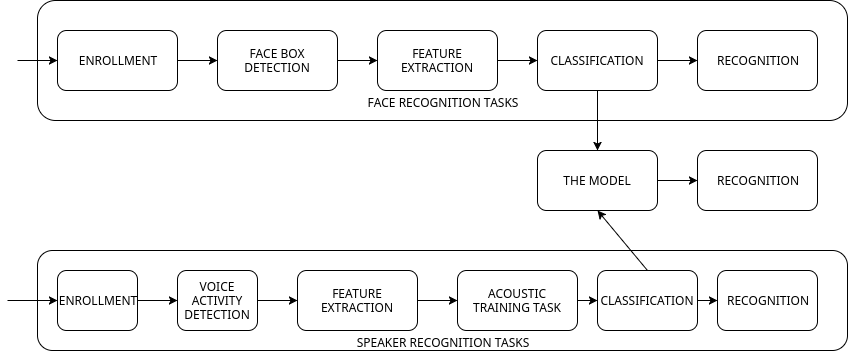
\includegraphics[width=5.5in]{./design.png}
% where an .eps filename suffix will be assumed under latex,
% and a .pdf suffix will be assumed for pdflatex; or what has been declared
% via \DeclareGraphicsExtensions.
\caption{Design}
\label{fig:High_Level_Design}
\end{figure}

%\begin{enumerate}
%  \item Design a function which takes the user voice through the microphone,
%        and the name of the user and returns True or False, accordingly.
%  \item Design a function which takes an image of the user, using the camera,
%        and the name of the user and returns True or False, accordingly.
%  \item Finally, design a system which unifies the functions designed above.
%        The system should be able:
%        \begin{itemize}
%          \item to override the default login screen in a GNU/Linux system.
%          \item to ensure the integrity of the confidential details created
%                using the above functions.
%        \end{itemize}
%\end{enumerate}

\chapter{Implementation, Result, and Analysis}


\section{Face Recognition}

\subsection{The EigenFace Approach}
Much of the previous work on automated face recognition has ignored the issue of
just what aspects of the face stimulus are important for identification.
This suggested that an information theory approach of encoding and decoding
face images may give insight into the information content of face images,
emphasizing the significant local and global features. Such features may or may not
be directly related to our intuitive notion of face features such as the eyes, nose,
lips, and hair. \\
In the language of information theory, the relevant information in a face image
should be extracted, encode it as efficiently as possible, and compare one face
encoding with a database of models encoded similarly. \\
A simple approach to extracting the information contained in an image of a face
is to somehow capture the variation in a collection of face images, independent
of any judgment of features, and use this information to encode and compare
individual face images. \\
In mathematical terms, we wish to find the principal components of the distribution of
faces, or the eigenvectors of the covariance matrix of the set of face images,
treating an image as a vector in a very high dimensional space. The eigenvectors
are ordered, each one accounting for a different amount of the variation among the face
images. \\
These eigenvectors can be thought of as a set of features that together characterize
the variation between face images. Each image location contributes more or less
to each eigenvector, so that the eigenvector is displayed as a sort of ghostly
face, which is called an eigenface (see Figure \ref{fig:meigenface}). \\
The approach to face recognition using the eigenface approach involves the
following initiation operations: \\
\begin{enumerate}
  \item Acquire an initial set of characteristic face images (the training set). \\
        This set should include a number of images for each person, with some
        variation in expression and in the lighting. \\
        (say \textbf{4} images of \textbf{10} people, so \textbf{M = 40}.)
  \item Calculate the eigenfaces from the training set, keeping only the M images
        that correspond to the highest eigenvalues. \\
        These M images define the \textit{face space}. As new faces are experienced,
        the eigenfaces can be updated or re-calculated.
        \begin{enumerate}
          \item Calculate the (M x M) matrix L, find it's eigenvectors and
                eigenvalues, and choose the M' eigenvectors with the highest
                associated eigenvalues. \\
                (Let $ M' = 10 $ in this example.)
          \item Combine the normalized training set of images (according to
                equation (\ref{eq:six})) to produce the (say, $ M' = 10 $) eigenfaces $ u_{k} $. \\
                \begin{equation} \label{eq:six}
                  u_{l} = \sum_{k = 1}^{M} v_{lk}\Phi_{k} \hspace{10 mm}, l = 1,2,\ldots,M
                \end{equation}
          \item For each known individual, calculate the class vector $ \Omega_{k} $
                by averaging the eigenface pattern vectors $ \Omega $ (from equation (\ref{eq:eight}))
                calculated from the original images (four, in this example) of the individual. \\
                \begin{equation} \label{eq:eight}
                  \epsilon_{k}^{2} = || (\Omega - \Omega_{k}) ||^{2}
                \end{equation}
                Choose a threshold $ \theta_{\epsilon} $ that defines the maximum
                allowable distance from any face class, and a threshold $ \theta_{\epsilon} $
                that defines the maximum allowable distance from face space.
                (according to equation (\ref{eq:nine})) \\
                \begin{equation} \label{eq:nine}
                  \epsilon^{2} = || (\Phi - \Phi_{f}) ||^{2}
                \end{equation}
          \item For each new face image to be identified, calculate it's pattern
                vector $ \Omega $, the distance $ \epsilon_{i} $ to each known
                class, and the distance $ \epsilon $ to face space. \\
                If the minimum distance $ \epsilon_{k} < \Theta_{\epsilon} $
                and the distance $ \epsilon < \Theta_{\epsilon} $, classify the
                input face as the individual associated with the class vector
                $ \Omega_{k} $. \\
                If the minimum distance $ \epsilon_{k} > \Theta_{\epsilon} $ but
                distance $ \epsilon < \Theta_{\epsilon} $, Then the image may be
                classified as unknown, and optionally used to begin a new face class.
        \end{enumerate}
  \item If the new image is classified as a known individual, this image may be added
        to the original set of familiar face images, and the eigenfaces may be recalculated
        (steps 1-2). This gives the opportunity to modify the face space as the
        system encounters more instances of known faces.
  \item Calculate the corresponding in M-dimensional weight space for each known
        individual, by projecting the face images onto the face space.
\end{enumerate}
The above initialization operations can be performed from time to time whenever
there is free excess computational capacity, available in the system. \\
Having initialized the system, the following steps are then used to recognize
new face images: \\
\begin{enumerate}
  \item Calculate a set of weights based on the input image and the M eigenfaces
        by projecting the input image onto each of the eigenfaces.
  \item Determine if the image is a face (whether known or unknown) by checking
        to see if the image is sufficiently close to face space.
  \item If it is a face, classify the weight pattern as either a known person or
        as unknown.
  \item Update the eigenfaces and/or weight pattern.
  \item If the same unknown face is seen several times, calculate its characteristic
        weight pattern and incorporate into the known faces.
\end{enumerate}

\begin{figure}[!t]
\centering
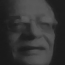
\includegraphics[width=1.5in]{./gulzar.png}
% where an .eps filename suffix will be assumed under latex,
% and a .pdf suffix will be assumed for pdflatex; or what has been declared
% via \DeclareGraphicsExtensions.
\caption{Mean Eigen Face}
\label{fig:meigenface}
\end{figure}

In the prototype implemented using the eigenfaces approach, calculation of the
eigenfaces is done as part of the training process. \\
The recognition, using the eigenfaces approach, takes about 90 seconds
implemented in Python on an Intel Core i5, using face images of size 132 x 132. \\

\subsection{The Local Binary Pattern Histogram Approach}
It is observed that if the above program is run without any alterations,
trained with a specific person, and another untrained face is introduced,
then it will be recognized as the trained person. \\
The methods to improve the accuracy of the Face Recognizer have been made more
stringent. The threshold used to control unknown faces, in the case of the
EigenFaceRecognizer, from the calculated distance can be adjusted to allow better
accuracy. A default of 2000 is used but by increasing this to 5000, for example,
will mean it will be less likely to allow a false match. \\

\subsection{Principle Component Analysis}
The EigenFaceRecognizer class applies PCA on each image, the results of which will
be an array of Eigen values that a neural network can be trained to recognize. \\
The LBPHFaceRecognizer uses Local Binary Patterns (LBP) to create a feature vector
using a Support Vector Machine or some other machine learning algorithm. \\

\subsection{The Local Binary Pattern Histogram Classifier}
The LBPH recognizer takes five variables: \\
\begin{description}
  \item[\textbf{radius}] \quad
  The radius used for building the Circular Local Binary Pattern.

  \item[\textbf{neighbors}] \quad
  The number of sample points to build a Circular Local Binary Pattern from.
  A value suggested by OpenCV documentation is eight sample points.
  The more the number of sample points, higher will be the computational cost.

  \item[\textbf{grid\_x}] \quad
  The number of cells in the horizontal direction.
  Eight is a common value used in publications.
  The more cells, the finer the grid, the higher the dimensionality of the
  resulting feature vector.

  \item[\textbf{grid\_y}] \quad
  The number of cells in the vertical direction.
  Eight is a common value used in publications.
  The more cells, the finer the grid, the higher the dimensionality of the
  resulting feature vector.

  \item[\textbf{threshold}] \quad
  The threshold applied in the prediction.
  If the distance to the nearest neighbor is larger than the threshold,
  the method returns \textbf{-1}.
\end{description}

\begin{figure}[!t]
\centering
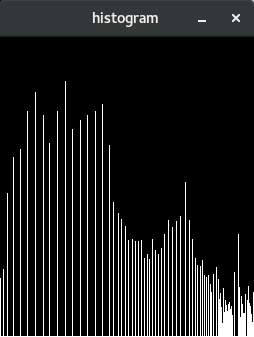
\includegraphics[width=1.5in]{./histogram.png}
% where an .eps filename suffix will be assumed under latex,
% and a .pdf suffix will be assumed for pdflatex; or what has been declared
% via \DeclareGraphicsExtensions.
\caption{Local Binary Pattern}
\label{fig:lbph}
\end{figure}

In the prototype implemented using the LBPH Approach (see Figure (\ref{fig:lbph})), calculation of the
LBP is done as part of the training process. \\
The recognition, using the LBPH approach, takes about 30 milliseconds
implemented in Python on an Intel Core i5, using face images of size 132 x 132. \\


\newpage


\section{Voice Recognition}

\subsection{Algorithm Used}
\begin{enumerate}
  \item An utterance of a user is collected during the enrollment procedure.
  \item Voice Activity Detection is performed: The silent part of the speech signals must be filtered out to decrease the bias that might occur during training.
  \item Feature Extraction
    \begin{itemize}
      \item Mel-Frequency Cepstral Coefficient (MFCC) is a representation of the short term power spectrum of a sound, based on a linear cosine transform of a log power spectrum on a non-linear mel-scale of frequency. This can be applied to speaker recognition task. The process to extract MFCC feature is demonstrated in Figure \ref{fig:MFCC_fig_one}. \\
      \begin{figure}[!t]
      \centering
      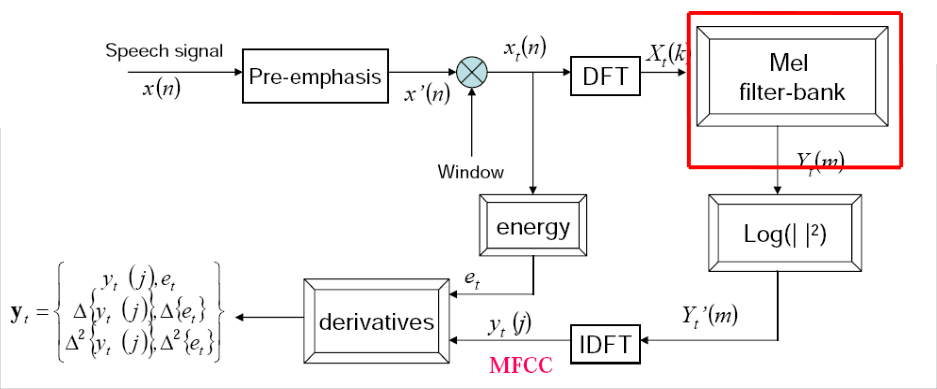
\includegraphics[width=2.5in]{./MFCC-mel-filterbank.png}
      % where an .eps filename suffix will be assumed under latex,
      % and a .pdf suffix will be assumed for pdflatex; or what has been declared
      % via \DeclareGraphicsExtensions.
      \caption{MFCC Feature Extraction Process}
      \label{fig:MFCC_fig_one}
      \end{figure}
      \\
      \item Linear Predictive Coding (LPC) is a tool used in audio signal processing and speech processing for representing the spectral envelope of a digital signal of speech in compressed form, using the information of a Linear predictive Model. \\
      The basic  assumption that is used in LPC is that, the n th signal is a linear combination of the previous p signals. An optimization can be done by the Levinson-Durbin algorithm, to estimate the coefficients ai in the signal, the squared error should be minimized.
    \end{itemize}
  \item Gaussian Mixture Model (GMM) is used in acoustic learning task such as speaker recognition, since it describes the varied distribution of all the feature vectors. Therefore, GMM is merely a weighted combination of multivariate Gaussian distribution which assumes feature vectors are independent. We use diagonal covariance since the dimensions of the feature vector is independent to each other. GMM can describe the distribution of feature vector with several clusters, as shown in Figure \ref{fig:GMM_fig_one}. \\
  \begin{figure}[!t]
  \centering
  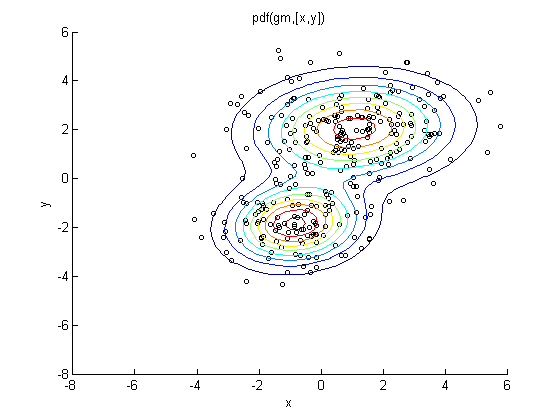
\includegraphics[width=2.5in]{./gmm.png}
  % where an .eps filename suffix will be assumed under latex,
  % and a .pdf suffix will be assumed for pdflatex; or what has been declared
  % via \DeclareGraphicsExtensions.
  \caption{A Two Dimensional GMM with Two Components}
  \label{fig:GMM_fig_one}
  \end{figure}
  \\
  After training, the model can give the score of fitness for every input feature vector, measuring the probability that the vector belongs to this model. Therefore in the task of speaker recognition, we can train a GMM for every speaker. Then for a input signal, we extract lists of feature vectors for it, and calculate the overall likelihood that the vector belongs to each model. The speaker whose model fits the input best will be chosen as the answer. \\
  Moreover, an enhancement has been done to the original GMM method. The training of GMM first requires a random initialization of the means of all the components. However, we can first use K-means algorithm to perform a clustering to all the vectors, then use the clustered centers to initialize the training of GMM. This enhancement can speed up the training and also give a better training result.
  \item Joint Factor Analysis (JFA) is a typical method which behave very well in classification problems, due to its ability to account for different types of variability in training data. Within all the factor analysis methods, JFA was proved to outperform other methods in the task of speaker recognition. \\  JFA models the user by supervector, i.e., a C x F dimension vector, where C is the number of components in the Universal Background Model, trained by GMM on all the training data, and F is the dimension of the acoustic feature vector. The supervector of an utterance is obtained by concatenating all the C means vectors in the trained GMM model.
\end{enumerate}


\section{The Biometric System}

\subsection{Advantages of Face Recognition}

\begin{enumerate}
  \item Face recognition systems are the least intrusive from a biometric sampling point of view because they neither require contact nor the awareness of the subject.
  \item The biometric works with legacy photograph databases, video tape and other image sources.
  \item It is a fairly good biometric identifier for small scale verification application.
\end{enumerate}

\subsection{Disadvantages of Face Recognition}

\begin{enumerate}
  \item A face needs to be well-lit by controled light sources in automated face authentication systems.
  \item Face is a poor biometric for use in a pure identification protocol, it performs better in verification.
\end{enumerate}

\subsection{Advantages of Voice Recognition}

\begin{enumerate}
  \item Voice is  natural biometric (one that people use instinctively to identify each other) under certain circumstances and machine decisions can be verified by relatively unskilled operators.
  \item The voice biometric requires only inexpensive hardware and is easily deployable over existing, ubiquitous communications infrastructure. Voice is therefor very suitable for pervasive security management.
  \item Voice allows incremental authentication protocols. For example, the protocol prescribes waiting for more voice data when a higher degree of recognition confidence is needed.
\end{enumerate}

\subsection{Disadvantages of Voice Recognition}

\begin{enumerate}
  \item Speech characterstics can drift away from models with age.
  \item With the improvement of text-to-speech technology improving, it becomes possible to create non-existent identities with machine voices and trainable speech synthesis may make it possible to create an automatic system that can imitate a given saying anything.
  \item Voice recognition is dependent on the quality of the captured audio signal. Speaker identification systems are susceptible to background noise, channel noise, and unknown channel or microphone characterstics.
\end{enumerate}
